\documentclass[a4paper]{amsart}
\usepackage[a4paper,margin=1in]{geometry}
\usepackage[T1]{fontenc}
\usepackage{lmodern,microtype,amssymb,graphicx,tikz}
\usepackage[hidelinks]{hyperref}
\usetikzlibrary{arrows.meta}

% styles of the three figures
\definecolor{bfS}{HTML}{0072B2}
\definecolor{bfW}{HTML}{009E73}
\colorlet{bfblack}{black!17}
\tikzset{
  bf/.style={line cap=round,line join=round,every node/.style={font=\footnotesize,inner sep=1.2pt}},
  bf edge/.style={draw=black!62,line width=.4pt},
  bf vertex/.style={fill=black},
  bf root/.style={draw=black,fill=white,line width=.7pt},
  bf D/.style={draw=bfS,line width=1.1pt,shorten >=1.6pt,shorten <=1.2pt,-{Stealth[length=4.2pt,width=3.6pt]}},
  bf spoke/.style={draw=black!70,line width=.4pt},
  bf kept/.style={draw=black,line width=1.1pt},
}

\newtheorem{theorem}{Theorem}
\newtheorem{proposition}[theorem]{Proposition}
\newtheorem{lemma}[theorem]{Lemma}

\newcommand{\eps}{\varepsilon}
\newcommand{\cP}{\mathcal P}

\title{Two sign-reversing involutions for the existence of a good state}
\author{}

\begin{document}

\begin{abstract}
The proof of Barnette's conjecture rests on the fact that an Eulerian triangulation with a pair of states has a good state.
In the paper that this note accompanies, this is proved by evaluating a generating function at $z=1$.
We give a bijective proof instead: two sign-reversing involutions on the set of pairs with $m$ marked crossings, where $m$ is the least number of cycles of a $2$-factor.
This is the argument sketched by Li in an appendix of his note on the proof, written out in full.
\end{abstract}

\maketitle

\section{Introduction}

This note accompanies the paper \emph{The proof of Barnette's conjecture}~\cite{P}, and it uses the notation and the terminology of that paper throughout.
So $T$ is an Eulerian triangulation with $n+1$ black faces, drawn with the black face $t_0$ as the unbounded face, $A$ is the set of the other black faces and $X$ the set of vertices other than the roots; we use states, good states and the graphs $Q_s$, pairs $(r,s)$ with the third corners $u(t)$ and the graphs $D(r,s)$, the graph $H$ and its $2$-factors $F$ with $c(F)$ cycles, the sign $\eps(r,s)$, the weight $\omega(s)$, and the number $a(C)$ of white faces inside a cycle $C$, all as defined in \cite[Sections~2 to~6]{P}.
We prove the following.

\begin{theorem}[{\cite[Proposition~6.9]{P}}]\label{main}
If $T$ has a pair, then $T$ has a good state.
\end{theorem}

In \cite{P} this is proved by showing that the Laurent polynomial $Z(z)=\sum_{(r,s)}\eps(r,s)z^{\omega(s)}$, to which only the pairs with a good second state contribute, is not zero: it is divisible by $(1-z)^m$, where $m$ is the least number of cycles of a $2$-factor of $H$, and the quotient takes at $z=1$ the value $\pm\Phi$, where
\begin{equation}\label{Phi}
\Phi=\sum_{F\,:\,c(F)=m}\ \prod_{C\in\mathcal C_F}a(C)
\end{equation}
is a positive integer.
Here we count instead.
The weight $\omega(s)$ is a signed number of points in which certain arcs $\gamma_y$ cross the arcs that represent $s$ in a drawing of $H$.
A \emph{marked pair} is a pair $(r,s)$ together with a set of $m$ of these crossings, and it has a sign.
We define two involutions on the set of marked pairs, each of which reverses the sign of every marked pair that it does not fix.
The first, $\iota_1$, keeps the second state and the marks; it is the involution of \cite[Lemma~5.6]{P}, and its fixed points are the marked pairs in which $s$ is good.
The second, $\iota_2$, either reverses a cycle of $D(r,s)$ or moves one mark along its arc $\gamma_y$; it has exactly $\Phi$ fixed points, and they all have the same sign.
So the signed number of marked pairs is $\pm\Phi\neq0$, and $\iota_1$ must have a fixed point.
Proposition~\ref{moment} shows that the signed number of marked pairs is $(-1)^m$ times the value of $Z(z)/(1-z)^m$ at $z=1$; the two involutions are thus a bijective form of the computation in~\cite{P}, with $\iota_2$ in the place of \cite[Lemma~6.6]{P} and of the product formula for $Z$.
Following the two involutions alternately from a fixed point of $\iota_2$ leads to a good state (Lemma~\ref{walk}).

The method is due to Li~\cite{Li}, who works in the dual graph $G$.
His objects correspond to our marked pairs, with vertical half-lines as the arcs $\gamma_y$, and his two involutions to $\iota_1$ and $\iota_2$.
Li carries out the case $m=1$, in which there is one mark, and he sketches the general case in his Appendix~B.
That appendix states the sign, the rule for a cycle without a mark, the rule for moving a mark, and the fixed points and their sign.
It does not prove that the map so described is an involution or that it reverses the sign, it does not say that the cycle has to be reversed when a mark whose white face lies inside its cycle moves to an arc of the first state, and it does not show that there is a fixed point when $m>1$, which needs an independent choice of direction for each cycle.
Lemmas~\ref{two} and~\ref{fixed} supply these steps for every $m$.
Li obtains a $2$-factor of $H$ under a connectivity assumption on $G$; Theorem~\ref{main} assumes only that $T$ has a pair, and \cite[Proposition~4.6]{P} gives one if $T$ has no separating triangle.

\section{Marked pairs}

We assume throughout that $T$ has a pair.
Then $H$ has a $2$-factor, and we let $m\ge1$ be the least number of cycles of a $2$-factor of $H$.

As in \cite[Section~6]{P}, we fix a point $p_t$ in every face $t\in A$ and arcs inside $t$ from $p_t$ to the corners of $t$ in $X$, which draw $H$ in the plane, and for every white face $y$ an arc $\gamma_y$ from a point of $y$ to a point of $t_0$.
The arc $\gamma_y$ avoids the vertices of $T$ and the points $p_t$, and it meets the arcs of $H$ in finitely many points, in each of which it crosses the arc of $H$.
A \emph{crossing} is a pair $x=(y,q)$ in which $q$ is a point of $\gamma_y$ on an arc of $H$.
If this arc joins $p_t$ to the corner $v$ of $t$, we say that $x$ \emph{lies on} this arc, and that $x$ is a crossing \emph{of} the state $s$ if $s(t)=v$.
Let $\chi(x)=1$ if $\gamma_y$ crosses the arc, directed from $p_t$ to $v$, from its left to its right in $q$, and $\chi(x)=-1$ otherwise.
The number $\chi(x)$ depends only on the crossing, not on a state.
By the definition of the local weights $\omega(t,v)$ in~\cite{P}, the weight of a state $s$ is
\begin{equation}\label{weight}
\omega(s)=\sum_{x}\chi(x),
\end{equation}
the sum being over the crossings of $s$.

A \emph{marked pair} is a triple $(r,s,\mu)$ in which $(r,s)$ is a pair and $\mu$ is a set of exactly $m$ crossings of $s$.
Different crossings in $\mu$ may belong to the same white face $y$, and they may lie on the same arc of $H$.
The set $\cP$ of all marked pairs is finite.
The \emph{sign} of a marked pair is
\[
\sigma(r,s,\mu)=\eps(r,s)\prod_{x\in\mu}\chi(x).
\]

Let $(r,s)$ be a pair with $2$-factor $F$, and let $C$ be a cycle of $D(r,s)$.
The corresponding cycle of $F$ is drawn as the closed curve $\Gamma$ that consists of the arcs from $p_t$ to $r(t)$ and to $s(t)$ for the faces $t$ with a side on $C$.
It is obtained from $C$ by pushing every edge of $C$ into its black face, and the region between an edge and its detour through $p_t$ lies in that face.
Hence, as in the proof of \cite[Lemma~6.6]{P}, $\Gamma$ is a simple closed curve with the same white faces inside as $C$, and when $\Gamma$ is run through from $r(t)$ to $p_t$ and on to $s(t)$ in each of these faces, it runs clockwise or counterclockwise as $C$ does.
We give $\Gamma$ this direction.
The curve $\Gamma$ depends only on $F$.
Reversing $C$ reverses the direction of $\Gamma$ and exchanges the arcs of $r$ and of $s$ on $\Gamma$, and it changes nothing on the other cycles of $F$.
We say that a cycle of $F$ \emph{carries} the crossings that lie on its arcs; every crossing of $s$ is carried by exactly one cycle of $F$.

\begin{lemma}\label{crossings}
Let $(r,s)$ be a pair, $C$ a cycle of $D(r,s)$ and $\Gamma$ the corresponding cycle of its $2$-factor.
Let $y$ be a white face, and let $x_1,\dots,x_k$ be the crossings of the form $(y,q)$ carried by $\Gamma$, in the order in which $\gamma_y$ passes through them, starting in $y$.
\begin{enumerate}
\item The number $k$ is odd if $y$ lies inside $C$, and even otherwise.
\item Let $1\le i<k$. If $x_i$ and $x_{i+1}$ lie both on arcs of $s$ or both on arcs of $r$, then $\chi(x_{i+1})=-\chi(x_i)$; if one of them lies on an arc of $s$ and the other on an arc of $r$, then $\chi(x_{i+1})=\chi(x_i)$.
\item If $y$ lies inside $C$ and $x_1$ lies on an arc of $s$, then $\chi(x_1)=1$ if $C$ runs counterclockwise, and $\chi(x_1)=-1$ if $C$ runs clockwise.
\end{enumerate}
\end{lemma}

\begin{proof}
The arc $\gamma_y$ meets $\Gamma$ exactly in the points of $x_1,\dots,x_k$, and it passes from one side of $\Gamma$ to the other in each of them.
It starts in $y$, which is inside $\Gamma$ if and only if it is inside $C$, and it ends in $t_0$, which is outside.
So $\gamma_y$ leaves and enters the inside of $\Gamma$ alternately, the last crossing leaves it, and this gives~(1); if $y$ is inside $C$, then $\gamma_y$ leaves the inside in $x_1$.
For a crossing $x$ carried by $\Gamma$ let $\lambda(x)=1$ if $\gamma_y$ crosses the directed curve $\Gamma$ from its left to its right, and $\lambda(x)=-1$ otherwise.
Then $\lambda(x_{i+1})=-\lambda(x_i)$.
The direction of $\Gamma$ is the direction away from $p_t$ on the arcs of $s$ and the direction towards $p_t$ on the arcs of $r$; so $\chi(x)=\lambda(x)$ if $x$ lies on an arc of $s$, and $\chi(x)=-\lambda(x)$ if $x$ lies on an arc of $r$.
This proves~(2).
If $C$ runs counterclockwise, then so does $\Gamma$, its inside is on its left, and $\lambda(x)=1$ where $\gamma_y$ leaves the inside; if $C$ runs clockwise, then $\lambda(x)=-1$ there.
This proves~(3).
\end{proof}

\section{The two involutions}

\subsection*{The first involution}
For every state $s$ such that $Q_s$ contains a cycle, choose one cycle $K_s$ of $Q_s$, as in the proof of \cite[Lemma~5.6]{P}.
For a marked pair $(r,s,\mu)$ put
\[
\iota_1(r,s,\mu)=\begin{cases}(r^{K_s},s,\mu)&\text{if $Q_s$ contains a cycle,}\\(r,s,\mu)&\text{otherwise,}\end{cases}
\]
where $r^K$ is the state that agrees with $r$ except that $r^K(t)=u(t)$ for the faces $t$ whose side in $Q_s$ lies on $K$.

\begin{lemma}\label{one}
The map $\iota_1$ is an involution on $\cP$.
Its fixed points are the marked pairs $(r,s,\mu)$ in which $s$ is good, and $\sigma(\iota_1(o))=-\sigma(o)$ for every other marked pair $o$.
\end{lemma}

\begin{proof}
Let $K=K_s$.
As shown in \cite[Lemma~5.5(2)]{P}, $r^K$ is a state, $(r^K,s)$ is a pair, and $(r^K)^K=r$.
The second state is unchanged; so $\mu$ is a set of crossings of the second state of $(r^K,s)$, the same cycle $K$ is chosen for the image, and $\iota_1$ is an involution.
A marked pair in which $Q_s$ contains a cycle is not fixed, because $r^K\ne r$, and its sign is reversed: $\eps(r^K,s)=-\eps(r,s)$ by \cite[Lemma~5.5(2)]{P}, and the numbers $\chi(x)$ are the same.
Finally, $Q_s$ contains no cycle if and only if $s$ is good, by \cite[Lemma~5.5(1)]{P}.
\end{proof}

\subsection*{The second involution}
Fix a total order on the set of all cycles of $H$; the \emph{first} cycle with some property is the first in this order.
Let $(r,s)$ be a pair with $2$-factor $F$, let $\Gamma$ be a cycle of $F$, $C$ the corresponding cycle of $D(r,s)$, and $y$ a white face.
List the crossings $(y,q)$ carried by $\Gamma$ as $x_1,\dots,x_k$, as in Lemma~\ref{crossings}.
If $y$ lies outside $C$, then $k$ is even, and we call $x_1$ and $x_2$, $x_3$ and $x_4$, and so on, \emph{partners}.
If $y$ lies inside $C$, then $k$ is odd; $x_1$ has no partner, and $x_2$ and $x_3$, $x_4$ and $x_5$, and so on, are partners.
The list and the partners depend only on $\Gamma$ and $y$, not on the pair.

For a marked pair $o=(r,s,\mu)$ with $2$-factor $F$ we define $\iota_2(o)$ by the first of the following rules that applies.
\begin{enumerate}
\item If some cycle of $F$ carries no crossing of $\mu$, let $\Gamma$ be the first such cycle, and let $(r',s')$ be obtained from $(r,s)$ by reversing the corresponding cycle of $D(r,s)$. Then $\iota_2(o)=(r',s',\mu)$.
\item Otherwise every cycle of $F$ carries a crossing of $\mu$. As $F$ has at least $m$ cycles and $\mu$ has $m$ elements, $F$ has exactly $m$ cycles, and each cycle $\Gamma$ carries exactly one crossing $x_\Gamma=(y_\Gamma,q_\Gamma)$ of $\mu$. If there is a cycle $\Gamma$ such that $y_\Gamma$ lies outside it, choose the first such cycle. If there is none, choose the first cycle $\Gamma$ such that $x_\Gamma$ is not the first crossing of $\gamma_{y_\Gamma}$ carried by $\Gamma$, that is, $x_\Gamma\ne x_1$ in the list for $\Gamma$ and $y_\Gamma$. If there is no such cycle either, then $\iota_2(o)=o$.
\item Let $\Gamma$ be the cycle chosen in (2), $x=x_\Gamma$, and let $x'$ be the partner of $x$. Put $\mu'=(\mu\setminus\{x\})\cup\{x'\}$. If $x'$ lies on an arc of $s$, then $\iota_2(o)=(r,s,\mu')$. If $x'$ lies on an arc of $r$, let $(r',s')$ be obtained from $(r,s)$ by reversing the cycle of $D(r,s)$ that corresponds to $\Gamma$; then $\iota_2(o)=(r',s',\mu')$.
\end{enumerate}
Here a white face lies inside or outside a cycle $\Gamma$ of $F$ according as it lies inside or outside the corresponding cycle of $D(r,s)$.
In (3) the crossing $x$ has a partner: if $y_\Gamma$ lies outside $\Gamma$ every crossing in the list has one, and otherwise $x\neq x_1$.

\begin{lemma}\label{two}
The map $\iota_2$ is an involution on $\cP$, and $\sigma(\iota_2(o))=-\sigma(o)$ for every marked pair $o$ that is not fixed.
The fixed points of $\iota_2$ are the marked pairs $(r,s,\mu)$ with the following property: the $2$-factor of $(r,s)$ has exactly $m$ cycles, and each of them carries exactly one crossing $(y,q)$ of $\mu$, for which $y$ lies inside the cycle and which is the first crossing of $\gamma_y$ carried by the cycle.
\end{lemma}

\begin{proof}
Let $o=(r,s,\mu)$ be a marked pair with $2$-factor $F$.
A pair obtained from $(r,s)$ by reversing a cycle has the same $2$-factor $F$, so the cycles of $F$, the crossings they carry and the white faces inside them are the same for $o$ and for $\iota_2(o)$ in all cases.

Suppose that rule (1) applies, to the cycle $\Gamma$.
The state $s'$ agrees with $s$ on all faces without an arc on $\Gamma$, and no crossing of $\mu$ is carried by $\Gamma$; so $\mu$ is a set of crossings of $s'$, and $(r',s',\mu)$ is a marked pair.
The same cycles of $F$ carry no crossing of $\mu$, so rule (1) applies to $\iota_2(o)$ with the same cycle $\Gamma$ and gives back $o$.
The pairs $(r,s)$ and $(r',s')$ have the same number of cycles, and the numbers of their counterclockwise cycles differ by one; so $\eps(r',s')=-\eps(r,s)$ by \cite[Lemma~6.2(3)]{P}, while the product of the $\chi(x)$ is the same.
Hence $\iota_2(o)\neq o$ and $\sigma(\iota_2(o))=-\sigma(o)$.

Suppose that rule (3) applies, to the cycle $\Gamma$ with the crossing $x$ and its partner $x'$.
The crossings of $\mu$ other than $x$ are carried by other cycles of $F$.
So they are different from $x'$, and they are crossings of the second state of $\iota_2(o)$, which agrees with $s$ on the faces without an arc on $\Gamma$.
The crossing $x'$ is a crossing of the second state of $\iota_2(o)$ as well: if it lies on an arc of $s$ the pair is not changed, and if it lies on an arc of $r$ then this arc belongs to $s'$.
Hence $\iota_2(o)$ is a marked pair, and every cycle of $F$ carries exactly one of its marked crossings.
For every cycle of $F$ this crossing belongs to the same white face as before.
So the first test in (2) chooses the same cycle $\Gamma$ for $\iota_2(o)$, if it chose $\Gamma$ for $o$.
If that test chooses no cycle, then $y_\Gamma$ lies inside $\Gamma$, both $x$ and $x'$ are different from the first crossing of $\gamma_{y_\Gamma}$ carried by $\Gamma$, the crossings on the other cycles are unchanged, and the second test again chooses $\Gamma$.
Therefore rule (3) applies to $\iota_2(o)$ with the same cycle $\Gamma$, and it moves the mark from $x'$ back to its partner $x$.
If the pair was not changed, then $x$ still lies on an arc of $s$, and the pair is not changed the second time.
If the cycle was reversed, then $x$ now lies on an arc of the first state $r'$, and the cycle is reversed again, which gives back $(r,s)$.
In both cases $\iota_2(\iota_2(o))=o$, and $\iota_2(o)\neq o$ because $\mu'\neq\mu$.

For the sign we use Lemma~\ref{crossings}(2); partners are consecutive in the list of that lemma.
If $x'$ lies on an arc of $s$, then so does $x$, hence $\chi(x')=-\chi(x)$, and the pair and the other crossings are unchanged.
If $x'$ lies on an arc of $r$, then $\chi(x')=\chi(x)$, since $x$ lies on an arc of $s$, and $\eps(r',s')=-\eps(r,s)$ as before.
In both cases $\sigma(\iota_2(o))=-\sigma(o)$.

So $o$ is fixed only if rule (2) applies and neither of its tests chooses a cycle, and this is the property stated in the lemma.
\end{proof}

\begin{lemma}\label{fixed}
The involution $\iota_2$ has exactly $\Phi$ fixed points, where $\Phi\ge1$ is the number defined in~\eqref{Phi}, and each of them has sign $(-1)^{(n-m)/2}$.
\end{lemma}

\begin{proof}
Let $F$ be a $2$-factor of $H$ with $m$ cycles, and choose for each cycle $\Gamma$ of $F$ a white face $y_\Gamma$ inside it; the same white face may be chosen for different cycles.
For each cycle there are $a(C)$ choices, where $C$ is the corresponding cycle of $D(r,s)$ for any pair $(r,s)$ with $2$-factor $F$, and $a(C)\ge1$ by \cite[Lemma~6.2(1)]{P}.
We show that exactly one fixed point of $\iota_2$ has the $2$-factor $F$ and these white faces; by Lemma~\ref{two} every fixed point arises in this way, so there are $\Phi$ of them.
By Lemma~\ref{crossings}(1), $\gamma_{y_\Gamma}$ has a first crossing $x_\Gamma$ carried by $\Gamma$, and by Lemma~\ref{two} the set $\mu$ of a fixed point must consist of these $m$ crossings, which are distinct because they are carried by distinct cycles.
The triple $(r,s,\mu)$ is a marked pair if and only if every $x_\Gamma$ lies on an arc of $s$.
The pairs with $2$-factor $F$ are obtained from one another by reversing cycles, which exchanges the arcs of $r$ and of $s$ on that cycle only; so exactly one of them has this property.

Let $(r,s,\mu)$ be a fixed point, and suppose that $c^+$ of the $m$ cycles of $D(r,s)$ run counterclockwise.
Then $\eps(r,s)=(-1)^{(n+m)/2+c^+}$ by \cite[Lemma~6.2(3)]{P}, and by Lemma~\ref{crossings}(3) the crossings of $\mu$ have $\chi(x)=1$ on the counterclockwise cycles and $\chi(x)=-1$ on the $m-c^+$ clockwise cycles.
So the sign is $(-1)^{(n+m)/2+m}=(-1)^{(n-m)/2}$.
\end{proof}

\begin{proof}[Proof of Theorem~\ref{main}]
By Lemma~\ref{two}, the marked pairs that are not fixed by $\iota_2$ cancel in pairs in the sum of the signs of all marked pairs; so by Lemma~\ref{fixed}
\begin{equation}\label{count}
\sum_{o\in\cP}\sigma(o)=(-1)^{(n-m)/2}\,\Phi\neq0.
\end{equation}
By Lemma~\ref{one}, the marked pairs that are not fixed by $\iota_1$ cancel in the same sum.
Hence $\iota_1$ has a fixed point $(r,s,\mu)$, and $s$ is a good state.
\end{proof}

\section{The relation to the polynomial $Z$}

\begin{proposition}\label{moment}
The Laurent polynomial $Z(z)=\sum_{(r,s)}\eps(r,s)z^{\omega(s)}$ of \cite{P} is divisible by $(1-z)^m$, and
\[
\sum_{o\in\cP}\sigma(o)\;=\;\frac1{m!}\sum_{(r,s)}\eps(r,s)\,\omega(s)^m\;=\;(-1)^m\,\frac{Z(z)}{(1-z)^m}\bigg|_{z=1},
\]
where the sums on the right are over all pairs.
\end{proposition}

\begin{proof}
Let $0\le j\le m$.
By~\eqref{weight}, $\omega(s)^j$ is the sum of the products $\chi(x_1)\cdots\chi(x_j)$ over all sequences $(x_1,\dots,x_j)$ of crossings of $s$, in which a crossing may occur several times.
So $\sum_{(r,s)}\eps(r,s)\omega(s)^j$ is a sum over the triples $(r,s,(x_1,\dots,x_j))$, each with the sign $\eps(r,s)\chi(x_1)\cdots\chi(x_j)$.
Consider the triples in which fewer than $m$ different crossings occur.
For such a triple some cycle of the $2$-factor of $(r,s)$ carries none of $x_1,\dots,x_j$, as there are at least $m$ cycles.
Reversing the first such cycle and keeping the sequence gives a triple of the same kind, and, as for rule (1) of $\iota_2$, this is an involution that reverses the sign.
Hence these triples cancel.
For $j<m$ these are all triples, and for $j=m$ the remaining triples are the $m!$ orderings of the sets $\mu$ of the marked pairs.
Therefore
\[
\sum_{(r,s)}\eps(r,s)\,\omega(s)^j=0\quad(j<m),\qquad \sum_{(r,s)}\eps(r,s)\,\omega(s)^m=m!\sum_{o\in\cP}\sigma(o).
\]
The $j$th derivative of $z^k$ at $z=1$ is $k(k-1)\cdots(k-j+1)$, for every integer $k$, and this is a polynomial in $k$ of degree $j$ with leading coefficient one.
So the derivatives of $Z$ of order less than $m$ vanish at $z=1$, and the $m$th derivative equals $\sum_{(r,s)}\eps(r,s)\omega(s)^m$ there.
Hence $Z(z)=(1-z)^mR(z)$ for a Laurent polynomial $R$, and $R(1)$ is $(-1)^m/m!$ times the $m$th derivative of $Z$ at $z=1$.
\end{proof}

With~\eqref{count} this gives the value $(-1)^{(n+m)/2}\Phi$ of $Z(z)/(1-z)^m$ at $z=1$ that is computed in the proof of \cite[Proposition~6.9]{P}.
There the cycles of each $2$-factor contribute the factors $1-z^{a(C)}$; here rule (1) of $\iota_2$ removes the terms that miss a cycle, and rule (3) leaves, for every cycle and every white face inside it, the first crossing of $\gamma_y$ and nothing else.

The number of marks has to be $m$.
With fewer than $m$ marks some cycle carries no mark, rule (1) always applies, and the signed number of marked pairs is zero, as in the proof of Proposition~\ref{moment}.
With more than $m$ marks a pair with $m$ cycles can have two marks on one cycle while every cycle carries a mark, and rule (3) is not defined.

The arcs $\gamma_y$ enter the proof only through the crossings, their order along each arc $\gamma_y$ and the numbers $\chi(x)$.
The set $\cP$ and the fixed points of the two involutions depend on the choice of the arcs, but the two sides of~\eqref{count} do not.
One can also choose the arcs without reference to a drawing.
For a white face $y$ take a path $y=f_0,f_1,\dots,f_j=t_0$ of distinct faces in which consecutive faces share a side, and let $\gamma_y$ pass through these faces in turn.
In a face $f_i\in A$ the sides by which $\gamma_y$ enters and leaves have a common corner $v$, and $\gamma_y$ can be drawn so that in $f_i$ it crosses the arc from $p_{f_i}$ to $v$ once and no other arc of $H$; it crosses no arc there if $v$ is a root.
The crossings are then the pairs $(y,i)$ with $f_i\in A$ and $v\in X$, such a crossing is a crossing of $s$ if $s(f_i)=v$, its place in the order along $\gamma_y$ is given by $i$, and $\chi(y,i)=1$ if $v$ lies to the left of the path at $f_i$, and $-1$ if it lies to the right.

\section{From a fixed point of the second involution to a good state}

The proof of Theorem~\ref{main} can be turned into a procedure.
Take a $2$-factor of $H$ with $m$ cycles and a white face inside each of its cycles, and let $o_0$ be the corresponding fixed point of $\iota_2$, as in the proof of Lemma~\ref{fixed}.
Put $o_1=\iota_1(o_0)$, $o_2=\iota_2(o_1)$, $o_3=\iota_1(o_2)$ and so on, and stop at the first $o_k$ that is fixed by the map that is to be applied to it.

\begin{lemma}\label{walk}
The marked pairs $o_0,o_1,\dots$ are distinct, the procedure stops, and the second state of the marked pair $o_k$ at which it stops is good.
\end{lemma}

\begin{proof}
Consider the graph on $\cP$ in which every marked pair $o$ that is not fixed by $\iota_i$ is joined to $\iota_i(o)$ by an edge with label $i$, for $i=1,2$; two marked pairs may be joined by two edges.
Every vertex lies on at most one edge of each label, and $o_0$ lies on no edge with label $2$.
So the component of $o_0$ is a path that begins in $o_0$, its edges have the labels $1,2,1,\dots$ in this order, and $o_0,\dots,o_k$ are its vertices.
If $k$ is odd, the last edge has label $1$ and $o_k$ is fixed by $\iota_2$; but $\sigma(o_k)=(-1)^k\sigma(o_0)=-\sigma(o_0)$ by Lemmas~\ref{one} and~\ref{two}, and this contradicts Lemma~\ref{fixed}.
Hence $k$ is even, $o_k$ is fixed by $\iota_1$, and its second state is good by Lemma~\ref{one}.
\end{proof}

This is the argument of the involution principle of Garsia and Milne~\cite{GM}.
The procedure takes at most $|\cP|-1$ steps, and it needs a $2$-factor with the least number of cycles to begin with.
A walk on pairs that alternates the two reversals of cycles also reaches a good state, and it starts from an arbitrary pair.

\section{An example}

Let $T$ be the triangulation of \cite[Figure~2]{P}, with $n=10$.
It has twelve states and eight pairs, and $H$ has two $2$-factors, each with two cycles; so $m=2$, and $\Phi=6\cdot1+3\cdot1=9$.
By~\eqref{count} the signed number of marked pairs is $9$, which is the value of $Z(z)/(1-z)^2=z^{\omega_0}\bigl((1+z+\dots+z^5)+z^2(1+z+z^2)\bigr)$ at $z=1$.
Figures~\ref{fig:marked} and~\ref{fig:second} show this triangulation in another drawing, with straight edges and with parallel segments as the arcs $\gamma_y$.
For these arcs there are $279$ marked pairs, in $273$ of which the second state is good.
Nine of them are fixed by $\iota_2$; they have sign $+1$, and in all nine the second state is good, so that the procedure of Lemma~\ref{walk} stops at once.
Figure~\ref{fig:first} shows the first involution in a triangulation with $m=1$.

\begin{figure}[tbp]
\centering
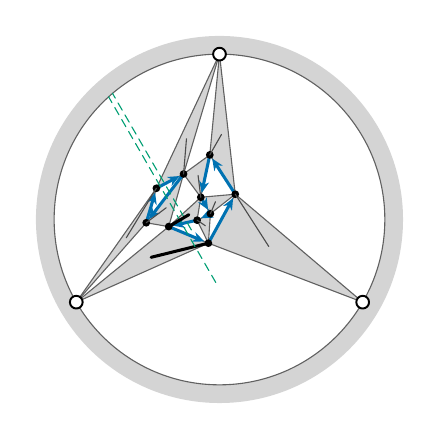
\begin{tikzpicture}[baseline=(current bounding box.center),bf,x=0.42cm,y=0.42cm]
\path[use as bounding box] (-5.80,-5.80) rectangle (5.80,5.80);
\fill[bfblack,even odd rule] (0,0) circle[radius=5.55] (0,0) circle[radius=5];
\fill[bfblack] (-0.335,-0.716) -- (-1.535,-0.215) -- (-4.330,-2.500) -- (-0.335,-0.716) -- cycle;
\fill[bfblack] (-2.215,-0.099) -- (-1.908,0.944) -- (-4.330,-2.500) -- (-2.215,-0.099) -- cycle;
\fill[bfblack] (-0.677,-0.021) -- (-0.565,0.672) -- (-1.535,-0.215) -- (-0.677,-0.021) -- cycle;
\fill[bfblack] (-1.086,1.376) -- (-2.215,-0.099) -- (-1.535,-0.215) -- (-1.086,1.376) -- cycle;
\fill[bfblack] (-1.086,1.376) -- (0.000,5.000) -- (-1.908,0.944) -- (-1.086,1.376) -- cycle;
\fill[bfblack] (-0.293,1.953) -- (0.477,0.764) -- (0.000,5.000) -- (-0.293,1.953) -- cycle;
\fill[bfblack] (0.477,0.764) -- (-0.335,-0.716) -- (4.330,-2.500) -- (0.477,0.764) -- cycle;
\fill[bfblack] (-0.275,0.175) -- (-0.677,-0.021) -- (-0.335,-0.716) -- (-0.275,0.175) -- cycle;
\fill[bfblack] (-0.275,0.175) -- (0.477,0.764) -- (-0.565,0.672) -- (-0.275,0.175) -- cycle;
\fill[bfblack] (-0.293,1.953) -- (-1.086,1.376) -- (-0.565,0.672) -- (-0.293,1.953) -- cycle;
\draw[bf edge] (0,0) circle[radius=5];
\draw[bf edge] (-4.330,-2.500) -- (-1.535,-0.215);
\draw[bf edge] (-4.330,-2.500) -- (-2.215,-0.099);
\draw[bf edge] (-4.330,-2.500) -- (-1.908,0.944);
\draw[bf edge] (-4.330,-2.500) -- (-0.335,-0.716);
\draw[bf edge] (-1.535,-0.215) -- (-2.215,-0.099);
\draw[bf edge] (-1.535,-0.215) -- (-0.335,-0.716);
\draw[bf edge] (-1.535,-0.215) -- (-0.677,-0.021);
\draw[bf edge] (-1.535,-0.215) -- (-0.565,0.672);
\draw[bf edge] (-1.535,-0.215) -- (-1.086,1.376);
\draw[bf edge] (-2.215,-0.099) -- (-1.908,0.944);
\draw[bf edge] (-2.215,-0.099) -- (-1.086,1.376);
\draw[bf edge] (-1.908,0.944) -- (0.000,5.000);
\draw[bf edge] (-1.908,0.944) -- (-1.086,1.376);
\draw[bf edge] (0.000,5.000) -- (-1.086,1.376);
\draw[bf edge] (0.000,5.000) -- (-0.293,1.953);
\draw[bf edge] (0.000,5.000) -- (0.477,0.764);
\draw[bf edge] (4.330,-2.500) -- (-0.335,-0.716);
\draw[bf edge] (4.330,-2.500) -- (0.477,0.764);
\draw[bf edge] (-0.335,-0.716) -- (-0.677,-0.021);
\draw[bf edge] (-0.335,-0.716) -- (0.477,0.764);
\draw[bf edge] (-0.335,-0.716) -- (-0.275,0.175);
\draw[bf edge] (-0.677,-0.021) -- (-0.565,0.672);
\draw[bf edge] (-0.677,-0.021) -- (-0.275,0.175);
\draw[bf edge] (-0.565,0.672) -- (-1.086,1.376);
\draw[bf edge] (-0.565,0.672) -- (-0.293,1.953);
\draw[bf edge] (-0.565,0.672) -- (0.477,0.764);
\draw[bf edge] (-0.565,0.672) -- (-0.275,0.175);
\draw[bf edge] (-1.086,1.376) -- (-0.293,1.953);
\draw[bf edge] (-0.293,1.953) -- (0.477,0.764);
\draw[bf edge] (0.477,0.764) -- (-0.275,0.175);
\draw[bf D] (-1.535,-0.215) -- (-0.335,-0.716);
\draw[bf D] (-2.215,-0.099) -- (-1.908,0.944);
\draw[bf D] (-0.677,-0.021) -- (-1.535,-0.215);
\draw[bf D] (-1.086,1.376) -- (-2.215,-0.099);
\draw[bf D] (-1.908,0.944) -- (-1.086,1.376);
\draw[bf D] (0.477,0.764) -- (-0.293,1.953);
\draw[bf D] (-0.335,-0.716) -- (0.477,0.764);
\draw[bf D] (-0.275,0.175) -- (-0.677,-0.021);
\draw[bf D] (-0.565,0.672) -- (-0.275,0.175);
\draw[bf D] (-0.293,1.953) -- (-0.565,0.672);
\draw[bf root] (-4.330,-2.500) circle[radius=2.3pt];
\fill[bf vertex] (-1.535,-0.215) circle[radius=1.4pt];
\fill[bf vertex] (-2.215,-0.099) circle[radius=1.4pt];
\fill[bf vertex] (-1.908,0.944) circle[radius=1.4pt];
\draw[bf root] (0.000,5.000) circle[radius=2.3pt];
\draw[bf root] (4.330,-2.500) circle[radius=2.3pt];
\fill[bf vertex] (-0.335,-0.716) circle[radius=1.4pt];
\fill[bf vertex] (-0.677,-0.021) circle[radius=1.4pt];
\fill[bf vertex] (-0.565,0.672) circle[radius=1.4pt];
\fill[bf vertex] (-1.086,1.376) circle[radius=1.4pt];
\fill[bf vertex] (-0.293,1.953) circle[radius=1.4pt];
\fill[bf vertex] (0.477,0.764) circle[radius=1.4pt];
\fill[bf vertex] (-0.275,0.175) circle[radius=1.4pt];
\draw[bf spoke] (-2.067,-1.144) -- (-0.335,-0.716);
\draw[bf spoke] (-2.817,-0.551) -- (-1.908,0.944);
\draw[bf spoke] (-0.926,0.145) -- (-1.535,-0.215);
\draw[bf spoke] (-1.612,0.354) -- (-2.215,-0.099);
\draw[bf spoke] (-0.998,2.440) -- (-1.086,1.376);
\draw[bf spoke] (0.061,2.572) -- (-0.293,1.953);
\draw[bf spoke] (1.491,-0.817) -- (0.477,0.764);
\draw[bf spoke] (-0.429,-0.188) -- (-0.677,-0.021);
\draw[bf spoke] (-0.121,0.537) -- (-0.275,0.175);
\draw[bf spoke] (-0.648,1.334) -- (-0.565,0.672);
\draw[bf kept] (-2.067,-1.144) -- (-0.335,-0.716);
\draw[bfW,densely dashed,thin] (-0.112,-1.905) -- (-3.353,3.709);
\draw[bfW,densely dashed,thin] (-0.849,-0.317) -- (-3.234,3.813);


\draw[bf kept] (-0.926,0.145) -- (-1.535,-0.215);


\end{tikzpicture}\qquad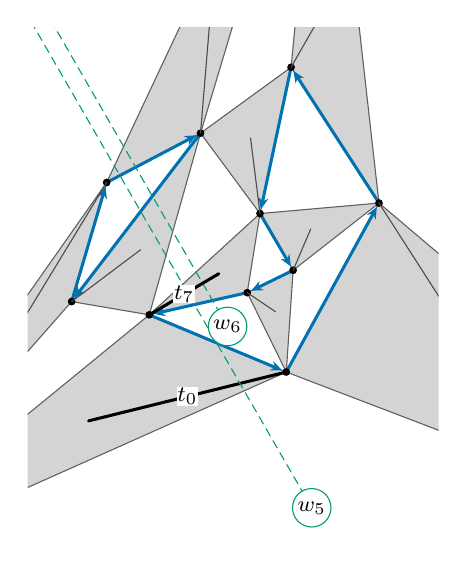
\begin{tikzpicture}[baseline=(current bounding box.center),bf,x=1.45cm,y=1.45cm]
\path[use as bounding box] (-2.6,-2.2) rectangle (1.0,2.3);\clip (-2.6,-2.2) rectangle (1.0,2.3);
\fill[bfblack,even odd rule] (0,0) circle[radius=5.55] (0,0) circle[radius=5];
\fill[bfblack] (-0.335,-0.716) -- (-1.535,-0.215) -- (-4.330,-2.500) -- (-0.335,-0.716) -- cycle;
\fill[bfblack] (-2.215,-0.099) -- (-1.908,0.944) -- (-4.330,-2.500) -- (-2.215,-0.099) -- cycle;
\fill[bfblack] (-0.677,-0.021) -- (-0.565,0.672) -- (-1.535,-0.215) -- (-0.677,-0.021) -- cycle;
\fill[bfblack] (-1.086,1.376) -- (-2.215,-0.099) -- (-1.535,-0.215) -- (-1.086,1.376) -- cycle;
\fill[bfblack] (-1.086,1.376) -- (0.000,5.000) -- (-1.908,0.944) -- (-1.086,1.376) -- cycle;
\fill[bfblack] (-0.293,1.953) -- (0.477,0.764) -- (0.000,5.000) -- (-0.293,1.953) -- cycle;
\fill[bfblack] (0.477,0.764) -- (-0.335,-0.716) -- (4.330,-2.500) -- (0.477,0.764) -- cycle;
\fill[bfblack] (-0.275,0.175) -- (-0.677,-0.021) -- (-0.335,-0.716) -- (-0.275,0.175) -- cycle;
\fill[bfblack] (-0.275,0.175) -- (0.477,0.764) -- (-0.565,0.672) -- (-0.275,0.175) -- cycle;
\fill[bfblack] (-0.293,1.953) -- (-1.086,1.376) -- (-0.565,0.672) -- (-0.293,1.953) -- cycle;
\draw[bf edge] (0,0) circle[radius=5];
\draw[bf edge] (-4.330,-2.500) -- (-1.535,-0.215);
\draw[bf edge] (-4.330,-2.500) -- (-2.215,-0.099);
\draw[bf edge] (-4.330,-2.500) -- (-1.908,0.944);
\draw[bf edge] (-4.330,-2.500) -- (-0.335,-0.716);
\draw[bf edge] (-1.535,-0.215) -- (-2.215,-0.099);
\draw[bf edge] (-1.535,-0.215) -- (-0.335,-0.716);
\draw[bf edge] (-1.535,-0.215) -- (-0.677,-0.021);
\draw[bf edge] (-1.535,-0.215) -- (-0.565,0.672);
\draw[bf edge] (-1.535,-0.215) -- (-1.086,1.376);
\draw[bf edge] (-2.215,-0.099) -- (-1.908,0.944);
\draw[bf edge] (-2.215,-0.099) -- (-1.086,1.376);
\draw[bf edge] (-1.908,0.944) -- (0.000,5.000);
\draw[bf edge] (-1.908,0.944) -- (-1.086,1.376);
\draw[bf edge] (0.000,5.000) -- (-1.086,1.376);
\draw[bf edge] (0.000,5.000) -- (-0.293,1.953);
\draw[bf edge] (0.000,5.000) -- (0.477,0.764);
\draw[bf edge] (4.330,-2.500) -- (-0.335,-0.716);
\draw[bf edge] (4.330,-2.500) -- (0.477,0.764);
\draw[bf edge] (-0.335,-0.716) -- (-0.677,-0.021);
\draw[bf edge] (-0.335,-0.716) -- (0.477,0.764);
\draw[bf edge] (-0.335,-0.716) -- (-0.275,0.175);
\draw[bf edge] (-0.677,-0.021) -- (-0.565,0.672);
\draw[bf edge] (-0.677,-0.021) -- (-0.275,0.175);
\draw[bf edge] (-0.565,0.672) -- (-1.086,1.376);
\draw[bf edge] (-0.565,0.672) -- (-0.293,1.953);
\draw[bf edge] (-0.565,0.672) -- (0.477,0.764);
\draw[bf edge] (-0.565,0.672) -- (-0.275,0.175);
\draw[bf edge] (-1.086,1.376) -- (-0.293,1.953);
\draw[bf edge] (-0.293,1.953) -- (0.477,0.764);
\draw[bf edge] (0.477,0.764) -- (-0.275,0.175);
\draw[bf D] (-1.535,-0.215) -- (-0.335,-0.716);
\draw[bf D] (-2.215,-0.099) -- (-1.908,0.944);
\draw[bf D] (-0.677,-0.021) -- (-1.535,-0.215);
\draw[bf D] (-1.086,1.376) -- (-2.215,-0.099);
\draw[bf D] (-1.908,0.944) -- (-1.086,1.376);
\draw[bf D] (0.477,0.764) -- (-0.293,1.953);
\draw[bf D] (-0.335,-0.716) -- (0.477,0.764);
\draw[bf D] (-0.275,0.175) -- (-0.677,-0.021);
\draw[bf D] (-0.565,0.672) -- (-0.275,0.175);
\draw[bf D] (-0.293,1.953) -- (-0.565,0.672);
\draw[bf root] (-4.330,-2.500) circle[radius=2.3pt];
\fill[bf vertex] (-1.535,-0.215) circle[radius=1.4pt];
\fill[bf vertex] (-2.215,-0.099) circle[radius=1.4pt];
\fill[bf vertex] (-1.908,0.944) circle[radius=1.4pt];
\draw[bf root] (0.000,5.000) circle[radius=2.3pt];
\draw[bf root] (4.330,-2.500) circle[radius=2.3pt];
\fill[bf vertex] (-0.335,-0.716) circle[radius=1.4pt];
\fill[bf vertex] (-0.677,-0.021) circle[radius=1.4pt];
\fill[bf vertex] (-0.565,0.672) circle[radius=1.4pt];
\fill[bf vertex] (-1.086,1.376) circle[radius=1.4pt];
\fill[bf vertex] (-0.293,1.953) circle[radius=1.4pt];
\fill[bf vertex] (0.477,0.764) circle[radius=1.4pt];
\fill[bf vertex] (-0.275,0.175) circle[radius=1.4pt];
\draw[bf spoke] (-2.067,-1.144) -- (-0.335,-0.716);
\draw[bf spoke] (-2.817,-0.551) -- (-1.908,0.944);
\draw[bf spoke] (-0.926,0.145) -- (-1.535,-0.215);
\draw[bf spoke] (-1.612,0.354) -- (-2.215,-0.099);
\draw[bf spoke] (-0.998,2.440) -- (-1.086,1.376);
\draw[bf spoke] (0.061,2.572) -- (-0.293,1.953);
\draw[bf spoke] (1.491,-0.817) -- (0.477,0.764);
\draw[bf spoke] (-0.429,-0.188) -- (-0.677,-0.021);
\draw[bf spoke] (-0.121,0.537) -- (-0.275,0.175);
\draw[bf spoke] (-0.648,1.334) -- (-0.565,0.672);
\draw[bf kept] (-2.067,-1.144) -- (-0.335,-0.716);
\draw[bfW,densely dashed,thin] (-0.112,-1.905) -- (-3.353,3.709);
\draw[bfW,densely dashed,thin] (-0.849,-0.317) -- (-3.234,3.813);
\node[draw=bfW,circle,fill=white,inner sep=1pt,font=\footnotesize] at (-0.112,-1.905) {$w_{5}$};
\node[fill=white,font=\footnotesize,inner sep=.3pt] at (-1.201,-0.930) {$t_{0}$};
\draw[bf kept] (-0.926,0.145) -- (-1.535,-0.215);
\node[draw=bfW,circle,fill=white,inner sep=1pt,font=\footnotesize] at (-0.849,-0.317) {$w_{6}$};
\node[fill=white,font=\footnotesize,inner sep=.3pt] at (-1.230,-0.035) {$t_{7}$};
\end{tikzpicture}
\caption{A marked pair $(r,s,\mu)$ in the triangulation of \cite[Figure~2]{P}. Left: the triangulation, with the roots drawn as circles and the edges of $D(r,s)$ as arrows; they form a cycle of length $7$ and a cycle of length $3$. Right: the same picture enlarged. The thin segment in each black face is the arc of $H$ to the corner chosen by $s$. The dashed lines are the arcs $\gamma_y$ and $\gamma_{y'}$. The two black dots are the crossings in $\mu$; they lie on the arcs of $s$ in the faces $t$ and $t'$, which are drawn thick. Both are carried by the cycle of the $2$-factor that corresponds to the cycle of length $7$. The other cycle carries no crossing of $\mu$, so $\iota_2$ reverses the cycle of length $3$ and keeps $\mu$.}
\label{fig:marked}
\end{figure}

\begin{figure}[tbp]
\centering
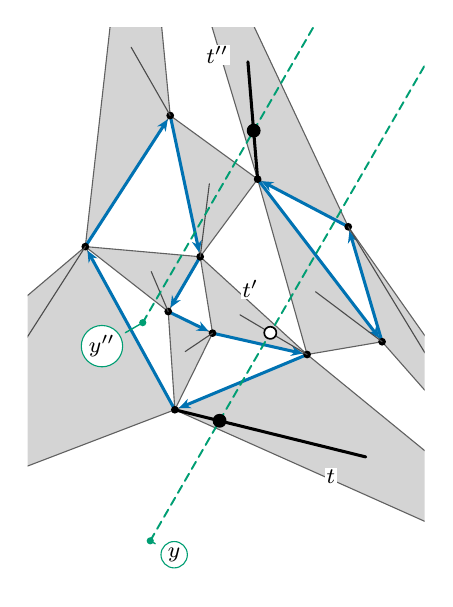
\begin{tikzpicture}[baseline=(current bounding box.center),bf,x=-1.4cm,y=1.4cm]
\path[use as bounding box] (-2.6,-2.25) rectangle (1.0,2.75);\clip (-2.6,-2.25) rectangle (1.0,2.75);
\fill[bfblack,even odd rule] (0,0) circle[radius=5.55] (0,0) circle[radius=5];
\fill[bfblack] (-0.335,-0.716) -- (-1.535,-0.215) -- (-4.330,-2.500) -- (-0.335,-0.716) -- cycle;
\fill[bfblack] (-2.215,-0.099) -- (-1.908,0.944) -- (-4.330,-2.500) -- (-2.215,-0.099) -- cycle;
\fill[bfblack] (-0.677,-0.021) -- (-0.565,0.672) -- (-1.535,-0.215) -- (-0.677,-0.021) -- cycle;
\fill[bfblack] (-1.086,1.376) -- (-2.215,-0.099) -- (-1.535,-0.215) -- (-1.086,1.376) -- cycle;
\fill[bfblack] (-1.086,1.376) -- (0.000,5.000) -- (-1.908,0.944) -- (-1.086,1.376) -- cycle;
\fill[bfblack] (-0.293,1.953) -- (0.477,0.764) -- (0.000,5.000) -- (-0.293,1.953) -- cycle;
\fill[bfblack] (0.477,0.764) -- (-0.335,-0.716) -- (4.330,-2.500) -- (0.477,0.764) -- cycle;
\fill[bfblack] (-0.275,0.175) -- (-0.677,-0.021) -- (-0.335,-0.716) -- (-0.275,0.175) -- cycle;
\fill[bfblack] (-0.275,0.175) -- (0.477,0.764) -- (-0.565,0.672) -- (-0.275,0.175) -- cycle;
\fill[bfblack] (-0.293,1.953) -- (-1.086,1.376) -- (-0.565,0.672) -- (-0.293,1.953) -- cycle;
\draw[bf edge] (0,0) circle[radius=5];
\draw[bf edge] (-4.330,-2.500) -- (-1.535,-0.215);
\draw[bf edge] (-4.330,-2.500) -- (-2.215,-0.099);
\draw[bf edge] (-4.330,-2.500) -- (-1.908,0.944);
\draw[bf edge] (-4.330,-2.500) -- (-0.335,-0.716);
\draw[bf edge] (-1.535,-0.215) -- (-2.215,-0.099);
\draw[bf edge] (-1.535,-0.215) -- (-0.335,-0.716);
\draw[bf edge] (-1.535,-0.215) -- (-0.677,-0.021);
\draw[bf edge] (-1.535,-0.215) -- (-0.565,0.672);
\draw[bf edge] (-1.535,-0.215) -- (-1.086,1.376);
\draw[bf edge] (-2.215,-0.099) -- (-1.908,0.944);
\draw[bf edge] (-2.215,-0.099) -- (-1.086,1.376);
\draw[bf edge] (-1.908,0.944) -- (0.000,5.000);
\draw[bf edge] (-1.908,0.944) -- (-1.086,1.376);
\draw[bf edge] (0.000,5.000) -- (-1.086,1.376);
\draw[bf edge] (0.000,5.000) -- (-0.293,1.953);
\draw[bf edge] (0.000,5.000) -- (0.477,0.764);
\draw[bf edge] (4.330,-2.500) -- (-0.335,-0.716);
\draw[bf edge] (4.330,-2.500) -- (0.477,0.764);
\draw[bf edge] (-0.335,-0.716) -- (-0.677,-0.021);
\draw[bf edge] (-0.335,-0.716) -- (0.477,0.764);
\draw[bf edge] (-0.335,-0.716) -- (-0.275,0.175);
\draw[bf edge] (-0.677,-0.021) -- (-0.565,0.672);
\draw[bf edge] (-0.677,-0.021) -- (-0.275,0.175);
\draw[bf edge] (-0.565,0.672) -- (-1.086,1.376);
\draw[bf edge] (-0.565,0.672) -- (-0.293,1.953);
\draw[bf edge] (-0.565,0.672) -- (0.477,0.764);
\draw[bf edge] (-0.565,0.672) -- (-0.275,0.175);
\draw[bf edge] (-1.086,1.376) -- (-0.293,1.953);
\draw[bf edge] (-0.293,1.953) -- (0.477,0.764);
\draw[bf edge] (0.477,0.764) -- (-0.275,0.175);
\draw[bf D] (-1.535,-0.215) -- (-0.335,-0.716);
\draw[bf D] (-2.215,-0.099) -- (-1.908,0.944);
\draw[bf D] (-0.677,-0.021) -- (-1.535,-0.215);
\draw[bf D] (-1.086,1.376) -- (-2.215,-0.099);
\draw[bf D] (-1.908,0.944) -- (-1.086,1.376);
\draw[bf D] (0.477,0.764) -- (-0.293,1.953);
\draw[bf D] (-0.335,-0.716) -- (0.477,0.764);
\draw[bf D] (-0.275,0.175) -- (-0.677,-0.021);
\draw[bf D] (-0.565,0.672) -- (-0.275,0.175);
\draw[bf D] (-0.293,1.953) -- (-0.565,0.672);
\draw[bf root] (-4.330,-2.500) circle[radius=2.3pt];
\fill[bf vertex] (-1.535,-0.215) circle[radius=1.4pt];
\fill[bf vertex] (-2.215,-0.099) circle[radius=1.4pt];
\fill[bf vertex] (-1.908,0.944) circle[radius=1.4pt];
\draw[bf root] (0.000,5.000) circle[radius=2.3pt];
\draw[bf root] (4.330,-2.500) circle[radius=2.3pt];
\fill[bf vertex] (-0.335,-0.716) circle[radius=1.4pt];
\fill[bf vertex] (-0.677,-0.021) circle[radius=1.4pt];
\fill[bf vertex] (-0.565,0.672) circle[radius=1.4pt];
\fill[bf vertex] (-1.086,1.376) circle[radius=1.4pt];
\fill[bf vertex] (-0.293,1.953) circle[radius=1.4pt];
\fill[bf vertex] (0.477,0.764) circle[radius=1.4pt];
\fill[bf vertex] (-0.275,0.175) circle[radius=1.4pt];
\draw[bf spoke] (-2.067,-1.144) -- (-0.335,-0.716);
\draw[bf spoke] (-2.817,-0.551) -- (-1.908,0.944);
\draw[bf spoke] (-0.926,0.145) -- (-1.535,-0.215);
\draw[bf spoke] (-1.612,0.354) -- (-2.215,-0.099);
\draw[bf spoke] (-0.998,2.440) -- (-1.086,1.376);
\draw[bf spoke] (0.061,2.572) -- (-0.293,1.953);
\draw[bf spoke] (1.491,-0.817) -- (0.477,0.764);
\draw[bf spoke] (-0.429,-0.188) -- (-0.677,-0.021);
\draw[bf spoke] (-0.121,0.537) -- (-0.275,0.175);
\draw[bf spoke] (-0.648,1.334) -- (-0.565,0.672);
\draw[bfW,densely dashed,line width=.7pt] (-0.112,-1.905) -- (-3.612,4.157);
\draw[bfW,densely dashed,line width=.7pt] (-0.044,0.074) -- (-3.544,6.136);
\draw[bf kept] (-2.067,-1.144) -- (-0.335,-0.716);
\draw[bf kept] (-0.998,2.440) -- (-1.086,1.376);
\draw[black,line width=.6pt,fill=black] (-0.741,-0.816) circle[radius=2.2pt];
\draw[black,line width=.6pt,fill=white] (-1.201,-0.018) circle[radius=2.2pt];
\draw[black,line width=.6pt,fill=black] (-1.050,1.816) circle[radius=2.2pt];
\draw[bfW,line width=.5pt] (-0.157,-1.931) -- (-0.112,-1.905);
\fill[bfW] (-0.112,-1.905) circle[radius=1.3pt];
\node[draw=bfW,circle,fill=white,inner sep=1pt,font=\footnotesize] at (-0.329,-2.031) {$y$};
\draw[bfW,line width=.5pt] (0.114,-0.017) -- (-0.044,0.074);
\fill[bfW] (-0.044,0.074) circle[radius=1.3pt];
\node[draw=bfW,circle,fill=white,inner sep=1pt,font=\footnotesize] at (0.326,-0.139) {$y''$};
\node[fill=white,font=\footnotesize,inner sep=.6pt] at (-1.750,-1.320) {$t$};
\node[fill=white,font=\footnotesize,inner sep=.6pt] at (-1.020,0.380) {$t'$};
\node[fill=white,font=\footnotesize,inner sep=.6pt] at (-0.720,2.500) {$t''$};
\end{tikzpicture}\quad$\longleftrightarrow$\quad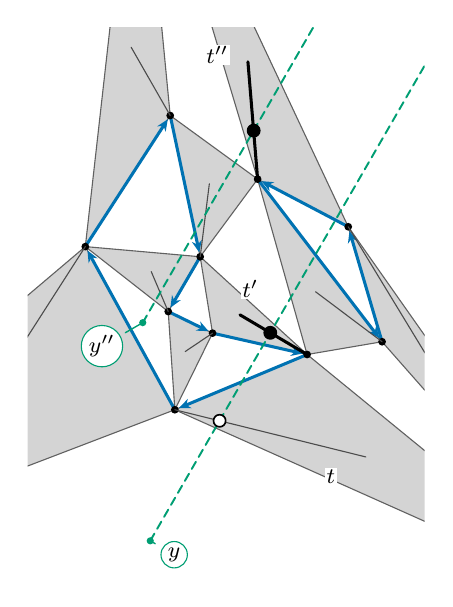
\begin{tikzpicture}[baseline=(current bounding box.center),bf,x=-1.4cm,y=1.4cm]
\path[use as bounding box] (-2.6,-2.25) rectangle (1.0,2.75);\clip (-2.6,-2.25) rectangle (1.0,2.75);
\fill[bfblack,even odd rule] (0,0) circle[radius=5.55] (0,0) circle[radius=5];
\fill[bfblack] (-0.335,-0.716) -- (-1.535,-0.215) -- (-4.330,-2.500) -- (-0.335,-0.716) -- cycle;
\fill[bfblack] (-2.215,-0.099) -- (-1.908,0.944) -- (-4.330,-2.500) -- (-2.215,-0.099) -- cycle;
\fill[bfblack] (-0.677,-0.021) -- (-0.565,0.672) -- (-1.535,-0.215) -- (-0.677,-0.021) -- cycle;
\fill[bfblack] (-1.086,1.376) -- (-2.215,-0.099) -- (-1.535,-0.215) -- (-1.086,1.376) -- cycle;
\fill[bfblack] (-1.086,1.376) -- (0.000,5.000) -- (-1.908,0.944) -- (-1.086,1.376) -- cycle;
\fill[bfblack] (-0.293,1.953) -- (0.477,0.764) -- (0.000,5.000) -- (-0.293,1.953) -- cycle;
\fill[bfblack] (0.477,0.764) -- (-0.335,-0.716) -- (4.330,-2.500) -- (0.477,0.764) -- cycle;
\fill[bfblack] (-0.275,0.175) -- (-0.677,-0.021) -- (-0.335,-0.716) -- (-0.275,0.175) -- cycle;
\fill[bfblack] (-0.275,0.175) -- (0.477,0.764) -- (-0.565,0.672) -- (-0.275,0.175) -- cycle;
\fill[bfblack] (-0.293,1.953) -- (-1.086,1.376) -- (-0.565,0.672) -- (-0.293,1.953) -- cycle;
\draw[bf edge] (0,0) circle[radius=5];
\draw[bf edge] (-4.330,-2.500) -- (-1.535,-0.215);
\draw[bf edge] (-4.330,-2.500) -- (-2.215,-0.099);
\draw[bf edge] (-4.330,-2.500) -- (-1.908,0.944);
\draw[bf edge] (-4.330,-2.500) -- (-0.335,-0.716);
\draw[bf edge] (-1.535,-0.215) -- (-2.215,-0.099);
\draw[bf edge] (-1.535,-0.215) -- (-0.335,-0.716);
\draw[bf edge] (-1.535,-0.215) -- (-0.677,-0.021);
\draw[bf edge] (-1.535,-0.215) -- (-0.565,0.672);
\draw[bf edge] (-1.535,-0.215) -- (-1.086,1.376);
\draw[bf edge] (-2.215,-0.099) -- (-1.908,0.944);
\draw[bf edge] (-2.215,-0.099) -- (-1.086,1.376);
\draw[bf edge] (-1.908,0.944) -- (0.000,5.000);
\draw[bf edge] (-1.908,0.944) -- (-1.086,1.376);
\draw[bf edge] (0.000,5.000) -- (-1.086,1.376);
\draw[bf edge] (0.000,5.000) -- (-0.293,1.953);
\draw[bf edge] (0.000,5.000) -- (0.477,0.764);
\draw[bf edge] (4.330,-2.500) -- (-0.335,-0.716);
\draw[bf edge] (4.330,-2.500) -- (0.477,0.764);
\draw[bf edge] (-0.335,-0.716) -- (-0.677,-0.021);
\draw[bf edge] (-0.335,-0.716) -- (0.477,0.764);
\draw[bf edge] (-0.335,-0.716) -- (-0.275,0.175);
\draw[bf edge] (-0.677,-0.021) -- (-0.565,0.672);
\draw[bf edge] (-0.677,-0.021) -- (-0.275,0.175);
\draw[bf edge] (-0.565,0.672) -- (-1.086,1.376);
\draw[bf edge] (-0.565,0.672) -- (-0.293,1.953);
\draw[bf edge] (-0.565,0.672) -- (0.477,0.764);
\draw[bf edge] (-0.565,0.672) -- (-0.275,0.175);
\draw[bf edge] (-1.086,1.376) -- (-0.293,1.953);
\draw[bf edge] (-0.293,1.953) -- (0.477,0.764);
\draw[bf edge] (0.477,0.764) -- (-0.275,0.175);
\draw[bf D] (-1.535,-0.215) -- (-0.335,-0.716);
\draw[bf D] (-2.215,-0.099) -- (-1.908,0.944);
\draw[bf D] (-0.677,-0.021) -- (-1.535,-0.215);
\draw[bf D] (-1.086,1.376) -- (-2.215,-0.099);
\draw[bf D] (-1.908,0.944) -- (-1.086,1.376);
\draw[bf D] (0.477,0.764) -- (-0.293,1.953);
\draw[bf D] (-0.335,-0.716) -- (0.477,0.764);
\draw[bf D] (-0.275,0.175) -- (-0.677,-0.021);
\draw[bf D] (-0.565,0.672) -- (-0.275,0.175);
\draw[bf D] (-0.293,1.953) -- (-0.565,0.672);
\draw[bf root] (-4.330,-2.500) circle[radius=2.3pt];
\fill[bf vertex] (-1.535,-0.215) circle[radius=1.4pt];
\fill[bf vertex] (-2.215,-0.099) circle[radius=1.4pt];
\fill[bf vertex] (-1.908,0.944) circle[radius=1.4pt];
\draw[bf root] (0.000,5.000) circle[radius=2.3pt];
\draw[bf root] (4.330,-2.500) circle[radius=2.3pt];
\fill[bf vertex] (-0.335,-0.716) circle[radius=1.4pt];
\fill[bf vertex] (-0.677,-0.021) circle[radius=1.4pt];
\fill[bf vertex] (-0.565,0.672) circle[radius=1.4pt];
\fill[bf vertex] (-1.086,1.376) circle[radius=1.4pt];
\fill[bf vertex] (-0.293,1.953) circle[radius=1.4pt];
\fill[bf vertex] (0.477,0.764) circle[radius=1.4pt];
\fill[bf vertex] (-0.275,0.175) circle[radius=1.4pt];
\draw[bf spoke] (-2.067,-1.144) -- (-0.335,-0.716);
\draw[bf spoke] (-2.817,-0.551) -- (-1.908,0.944);
\draw[bf spoke] (-0.926,0.145) -- (-1.535,-0.215);
\draw[bf spoke] (-1.612,0.354) -- (-2.215,-0.099);
\draw[bf spoke] (-0.998,2.440) -- (-1.086,1.376);
\draw[bf spoke] (0.061,2.572) -- (-0.293,1.953);
\draw[bf spoke] (1.491,-0.817) -- (0.477,0.764);
\draw[bf spoke] (-0.429,-0.188) -- (-0.677,-0.021);
\draw[bf spoke] (-0.121,0.537) -- (-0.275,0.175);
\draw[bf spoke] (-0.648,1.334) -- (-0.565,0.672);
\draw[bfW,densely dashed,line width=.7pt] (-0.112,-1.905) -- (-3.612,4.157);
\draw[bfW,densely dashed,line width=.7pt] (-0.044,0.074) -- (-3.544,6.136);
\draw[bf kept] (-0.926,0.145) -- (-1.535,-0.215);
\draw[bf kept] (-0.998,2.440) -- (-1.086,1.376);
\draw[black,line width=.6pt,fill=white] (-0.741,-0.816) circle[radius=2.2pt];
\draw[black,line width=.6pt,fill=black] (-1.201,-0.018) circle[radius=2.2pt];
\draw[black,line width=.6pt,fill=black] (-1.050,1.816) circle[radius=2.2pt];
\draw[bfW,line width=.5pt] (-0.157,-1.931) -- (-0.112,-1.905);
\fill[bfW] (-0.112,-1.905) circle[radius=1.3pt];
\node[draw=bfW,circle,fill=white,inner sep=1pt,font=\footnotesize] at (-0.329,-2.031) {$y$};
\draw[bfW,line width=.5pt] (0.114,-0.017) -- (-0.044,0.074);
\fill[bfW] (-0.044,0.074) circle[radius=1.3pt];
\node[draw=bfW,circle,fill=white,inner sep=1pt,font=\footnotesize] at (0.326,-0.139) {$y''$};
\node[fill=white,font=\footnotesize,inner sep=.6pt] at (-1.750,-1.320) {$t$};
\node[fill=white,font=\footnotesize,inner sep=.6pt] at (-1.020,0.380) {$t'$};
\node[fill=white,font=\footnotesize,inner sep=.6pt] at (-0.720,2.500) {$t''$};
\end{tikzpicture}

\caption{The second involution moves a mark. Left: the pair $(r,s)$ of Figure~\ref{fig:marked} with the crossings of $\gamma_y$ in $t$ and of $\gamma_{y''}$ in $t''$ as marks (black dots). Each of the two cycles of the $2$-factor carries one of them. The face $y$ lies outside the cycle of length $7$, and $\gamma_y$ meets the corresponding cycle of the $2$-factor twice, on the arcs of $s$ in $t$ and in $t'$; these two crossings are partners. Right: the image under $\iota_2$, when this cycle is the first. The mark has moved along $\gamma_y$ to the partner; the hollow dot is the crossing without the mark. Both arcs belong to $s$, so no cycle is reversed, and the sign changes because the two crossings have different values of $\chi$.}
\label{fig:second}
\end{figure}

\begin{figure}[tbp]
\centering
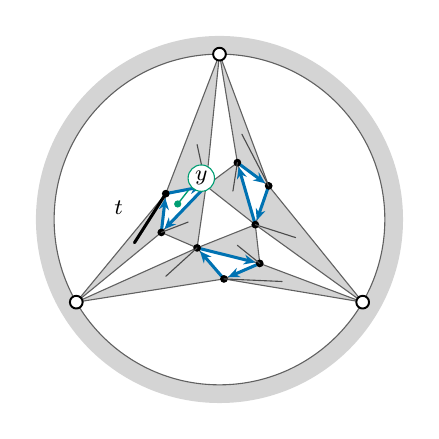
\begin{tikzpicture}[baseline=(current bounding box.center),bf,x=0.42cm,y=0.42cm]
\path[use as bounding box] (-5.80,-5.80) rectangle (5.80,5.80);
\fill[bfblack,even odd rule] (0,0) circle[radius=5.55] (0,0) circle[radius=5];
\fill[bfblack] (-4.330,-2.500) -- (-1.759,-0.391) -- (-1.624,0.781) -- (-4.330,-2.500) -- cycle;
\fill[bfblack] (-0.406,1.016) -- (0.000,5.000) -- (-1.624,0.781) -- (-0.406,1.016) -- cycle;
\fill[bfblack] (-0.677,-0.859) -- (-0.406,1.016) -- (-1.759,-0.391) -- (-0.677,-0.859) -- cycle;
\fill[bfblack] (0.135,-1.797) -- (-0.677,-0.859) -- (-4.330,-2.500) -- (0.135,-1.797) -- cycle;
\fill[bfblack] (0.541,1.719) -- (1.488,1.016) -- (0.000,5.000) -- (0.541,1.719) -- cycle;
\fill[bfblack] (1.083,-0.156) -- (0.541,1.719) -- (-0.406,1.016) -- (1.083,-0.156) -- cycle;
\fill[bfblack] (1.218,-1.328) -- (1.083,-0.156) -- (-0.677,-0.859) -- (1.218,-1.328) -- cycle;
\fill[bfblack] (4.330,-2.500) -- (1.218,-1.328) -- (0.135,-1.797) -- (4.330,-2.500) -- cycle;
\fill[bfblack] (1.488,1.016) -- (1.083,-0.156) -- (4.330,-2.500) -- (1.488,1.016) -- cycle;
\draw[bf edge] (0,0) circle[radius=5];
\draw[bf edge] (-1.624,0.781) -- (-1.759,-0.391);
\draw[bf edge] (-1.624,0.781) -- (-4.330,-2.500);
\draw[bf edge] (-1.624,0.781) -- (0.000,5.000);
\draw[bf edge] (-1.624,0.781) -- (-0.406,1.016);
\draw[bf edge] (-1.759,-0.391) -- (-4.330,-2.500);
\draw[bf edge] (-1.759,-0.391) -- (-0.406,1.016);
\draw[bf edge] (-1.759,-0.391) -- (-0.677,-0.859);
\draw[bf edge] (-4.330,-2.500) -- (-0.677,-0.859);
\draw[bf edge] (-4.330,-2.500) -- (0.135,-1.797);
\draw[bf edge] (0.000,5.000) -- (-0.406,1.016);
\draw[bf edge] (0.000,5.000) -- (1.488,1.016);
\draw[bf edge] (0.000,5.000) -- (0.541,1.719);
\draw[bf edge] (-0.406,1.016) -- (-0.677,-0.859);
\draw[bf edge] (-0.406,1.016) -- (0.541,1.719);
\draw[bf edge] (-0.406,1.016) -- (1.083,-0.156);
\draw[bf edge] (-0.677,-0.859) -- (0.135,-1.797);
\draw[bf edge] (-0.677,-0.859) -- (1.083,-0.156);
\draw[bf edge] (-0.677,-0.859) -- (1.218,-1.328);
\draw[bf edge] (0.135,-1.797) -- (4.330,-2.500);
\draw[bf edge] (0.135,-1.797) -- (1.218,-1.328);
\draw[bf edge] (4.330,-2.500) -- (1.488,1.016);
\draw[bf edge] (4.330,-2.500) -- (1.083,-0.156);
\draw[bf edge] (4.330,-2.500) -- (1.218,-1.328);
\draw[bf edge] (1.488,1.016) -- (0.541,1.719);
\draw[bf edge] (1.488,1.016) -- (1.083,-0.156);
\draw[bf edge] (0.541,1.719) -- (1.083,-0.156);
\draw[bf edge] (1.083,-0.156) -- (1.218,-1.328);
\draw[bf D] (-1.759,-0.391) -- (-1.624,0.781);
\draw[bf D] (-1.624,0.781) -- (-0.406,1.016);
\draw[bf D] (-0.406,1.016) -- (-1.759,-0.391);
\draw[bf D] (0.135,-1.797) -- (-0.677,-0.859);
\draw[bf D] (0.541,1.719) -- (1.488,1.016);
\draw[bf D] (1.083,-0.156) -- (0.541,1.719);
\draw[bf D] (-0.677,-0.859) -- (1.218,-1.328);
\draw[bf D] (1.218,-1.328) -- (0.135,-1.797);
\draw[bf D] (1.488,1.016) -- (1.083,-0.156);
\fill[bf vertex] (-1.624,0.781) circle[radius=1.4pt];
\fill[bf vertex] (-1.759,-0.391) circle[radius=1.4pt];
\draw[bf root] (-4.330,-2.500) circle[radius=2.3pt];
\draw[bf root] (0.000,5.000) circle[radius=2.3pt];
\fill[bf vertex] (-0.406,1.016) circle[radius=1.4pt];
\fill[bf vertex] (-0.677,-0.859) circle[radius=1.4pt];
\fill[bf vertex] (0.135,-1.797) circle[radius=1.4pt];
\draw[bf root] (4.330,-2.500) circle[radius=2.3pt];
\fill[bf vertex] (1.488,1.016) circle[radius=1.4pt];
\fill[bf vertex] (0.541,1.719) circle[radius=1.4pt];
\fill[bf vertex] (1.083,-0.156) circle[radius=1.4pt];
\fill[bf vertex] (1.218,-1.328) circle[radius=1.4pt];
\draw[bf spoke] (-2.571,-0.703) -- (-1.624,0.781);
\draw[bf spoke] (-0.677,2.266) -- (-0.406,1.016);
\draw[bf spoke] (-0.947,-0.078) -- (-1.759,-0.391);
\draw[bf spoke] (-1.624,-1.719) -- (-0.677,-0.859);
\draw[bf spoke] (0.677,2.578) -- (1.488,1.016);
\draw[bf spoke] (0.406,0.859) -- (0.541,1.719);
\draw[bf spoke] (0.541,-0.781) -- (1.218,-1.328);
\draw[bf spoke] (1.894,-1.875) -- (0.135,-1.797);
\draw[bf spoke] (2.300,-0.547) -- (1.083,-0.156);
\draw[bf kept] (-2.571,-0.703) -- (-1.624,0.781);
\node[draw=bfW,circle,fill=white,inner sep=1pt,font=\footnotesize] at (-0.550,1.250) {$y$};
\draw[bfW,line width=.5pt] (-0.95,0.87) -- (-1.263,0.469);
\fill[bfW] (-1.263,0.469) circle[radius=1.3pt];
\node[fill=white,font=\footnotesize,inner sep=.3pt] at (-3.050,0.350) {$t$};
\end{tikzpicture}\quad$\longleftrightarrow$\quad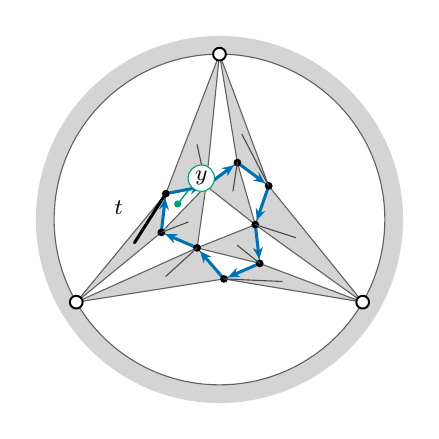
\begin{tikzpicture}[baseline=(current bounding box.center),bf,x=0.42cm,y=0.42cm]
\path[use as bounding box] (-5.80,-5.80) rectangle (5.80,5.80);
\fill[bfblack,even odd rule] (0,0) circle[radius=5.55] (0,0) circle[radius=5];
\fill[bfblack] (-4.330,-2.500) -- (-1.759,-0.391) -- (-1.624,0.781) -- (-4.330,-2.500) -- cycle;
\fill[bfblack] (-0.406,1.016) -- (0.000,5.000) -- (-1.624,0.781) -- (-0.406,1.016) -- cycle;
\fill[bfblack] (-0.677,-0.859) -- (-0.406,1.016) -- (-1.759,-0.391) -- (-0.677,-0.859) -- cycle;
\fill[bfblack] (0.135,-1.797) -- (-0.677,-0.859) -- (-4.330,-2.500) -- (0.135,-1.797) -- cycle;
\fill[bfblack] (0.541,1.719) -- (1.488,1.016) -- (0.000,5.000) -- (0.541,1.719) -- cycle;
\fill[bfblack] (1.083,-0.156) -- (0.541,1.719) -- (-0.406,1.016) -- (1.083,-0.156) -- cycle;
\fill[bfblack] (1.218,-1.328) -- (1.083,-0.156) -- (-0.677,-0.859) -- (1.218,-1.328) -- cycle;
\fill[bfblack] (4.330,-2.500) -- (1.218,-1.328) -- (0.135,-1.797) -- (4.330,-2.500) -- cycle;
\fill[bfblack] (1.488,1.016) -- (1.083,-0.156) -- (4.330,-2.500) -- (1.488,1.016) -- cycle;
\draw[bf edge] (0,0) circle[radius=5];
\draw[bf edge] (-1.624,0.781) -- (-1.759,-0.391);
\draw[bf edge] (-1.624,0.781) -- (-4.330,-2.500);
\draw[bf edge] (-1.624,0.781) -- (0.000,5.000);
\draw[bf edge] (-1.624,0.781) -- (-0.406,1.016);
\draw[bf edge] (-1.759,-0.391) -- (-4.330,-2.500);
\draw[bf edge] (-1.759,-0.391) -- (-0.406,1.016);
\draw[bf edge] (-1.759,-0.391) -- (-0.677,-0.859);
\draw[bf edge] (-4.330,-2.500) -- (-0.677,-0.859);
\draw[bf edge] (-4.330,-2.500) -- (0.135,-1.797);
\draw[bf edge] (0.000,5.000) -- (-0.406,1.016);
\draw[bf edge] (0.000,5.000) -- (1.488,1.016);
\draw[bf edge] (0.000,5.000) -- (0.541,1.719);
\draw[bf edge] (-0.406,1.016) -- (-0.677,-0.859);
\draw[bf edge] (-0.406,1.016) -- (0.541,1.719);
\draw[bf edge] (-0.406,1.016) -- (1.083,-0.156);
\draw[bf edge] (-0.677,-0.859) -- (0.135,-1.797);
\draw[bf edge] (-0.677,-0.859) -- (1.083,-0.156);
\draw[bf edge] (-0.677,-0.859) -- (1.218,-1.328);
\draw[bf edge] (0.135,-1.797) -- (4.330,-2.500);
\draw[bf edge] (0.135,-1.797) -- (1.218,-1.328);
\draw[bf edge] (4.330,-2.500) -- (1.488,1.016);
\draw[bf edge] (4.330,-2.500) -- (1.083,-0.156);
\draw[bf edge] (4.330,-2.500) -- (1.218,-1.328);
\draw[bf edge] (1.488,1.016) -- (0.541,1.719);
\draw[bf edge] (1.488,1.016) -- (1.083,-0.156);
\draw[bf edge] (0.541,1.719) -- (1.083,-0.156);
\draw[bf edge] (1.083,-0.156) -- (1.218,-1.328);
\draw[bf D] (-1.759,-0.391) -- (-1.624,0.781);
\draw[bf D] (-1.624,0.781) -- (-0.406,1.016);
\draw[bf D] (-0.677,-0.859) -- (-1.759,-0.391);
\draw[bf D] (0.135,-1.797) -- (-0.677,-0.859);
\draw[bf D] (0.541,1.719) -- (1.488,1.016);
\draw[bf D] (-0.406,1.016) -- (0.541,1.719);
\draw[bf D] (1.083,-0.156) -- (1.218,-1.328);
\draw[bf D] (1.218,-1.328) -- (0.135,-1.797);
\draw[bf D] (1.488,1.016) -- (1.083,-0.156);
\fill[bf vertex] (-1.624,0.781) circle[radius=1.4pt];
\fill[bf vertex] (-1.759,-0.391) circle[radius=1.4pt];
\draw[bf root] (-4.330,-2.500) circle[radius=2.3pt];
\draw[bf root] (0.000,5.000) circle[radius=2.3pt];
\fill[bf vertex] (-0.406,1.016) circle[radius=1.4pt];
\fill[bf vertex] (-0.677,-0.859) circle[radius=1.4pt];
\fill[bf vertex] (0.135,-1.797) circle[radius=1.4pt];
\draw[bf root] (4.330,-2.500) circle[radius=2.3pt];
\fill[bf vertex] (1.488,1.016) circle[radius=1.4pt];
\fill[bf vertex] (0.541,1.719) circle[radius=1.4pt];
\fill[bf vertex] (1.083,-0.156) circle[radius=1.4pt];
\fill[bf vertex] (1.218,-1.328) circle[radius=1.4pt];
\draw[bf spoke] (-2.571,-0.703) -- (-1.624,0.781);
\draw[bf spoke] (-0.677,2.266) -- (-0.406,1.016);
\draw[bf spoke] (-0.947,-0.078) -- (-1.759,-0.391);
\draw[bf spoke] (-1.624,-1.719) -- (-0.677,-0.859);
\draw[bf spoke] (0.677,2.578) -- (1.488,1.016);
\draw[bf spoke] (0.406,0.859) -- (0.541,1.719);
\draw[bf spoke] (0.541,-0.781) -- (1.218,-1.328);
\draw[bf spoke] (1.894,-1.875) -- (0.135,-1.797);
\draw[bf spoke] (2.300,-0.547) -- (1.083,-0.156);
\draw[bf kept] (-2.571,-0.703) -- (-1.624,0.781);
\node[draw=bfW,circle,fill=white,inner sep=1pt,font=\footnotesize] at (-0.550,1.250) {$y$};
\draw[bfW,line width=.5pt] (-0.95,0.87) -- (-1.263,0.469);
\fill[bfW] (-1.263,0.469) circle[radius=1.3pt];
\node[fill=white,font=\footnotesize,inner sep=.3pt] at (-3.050,0.350) {$t$};
\end{tikzpicture}
\caption{The first involution, in an Eulerian triangulation with $12$ vertices in which $m=1$. The two marked pairs have the same second state $s$ and the same mark, a crossing of $\gamma_y$ on the arc of $s$ in the face $t$; this arc is drawn thick, and $\gamma_y$ is not drawn. The first state differs on the faces with a side on a cycle of $Q_s$, so the arrows of $D(r,s)$ differ between the two panels.}
\label{fig:first}
\end{figure}

\begin{thebibliography}{9}

\bibitem{GM}
A.~M. Garsia and S.~C. Milne, \emph{A Rogers--Ramanujan bijection}, J. Combin. Theory Ser. A \textbf{31} (1981), 289--339.

\bibitem{Li}
Z.~Li, \emph{A note on the proof of Barnette's conjecture}, preprint, arXiv:2610.30490, 2026.

\bibitem{P}
\emph{The proof of Barnette's conjecture}, the paper that this note accompanies.

\end{thebibliography}

\end{document}
